\chapter{Methodology}
\index{Methodology@\emph{Methodology}}%
\label{chap:methodology}

\section{Overview}\label{sec:method overview}

To examine the effects of cooperativity conscious schedulers we needed to have 
a method for comparing several scheduler implementations without needing to 
modify the underlying implementation of processes, channels, or application
source code. It would be also beneficial if our solution were able to visualize
these differences similar to Haskell's ThreadScope \cite{jones2009parallel}.

Our solution, $ErLam$, is a compiler for an experimental version of Lambda 
Calculus with Swap Channels and a runtime system which allows for swappable 
scheduler mechanisms and an optional logging system which can be fed into a 
custom report generator.
We break up our solution description into three parts; 
Section~\ref{sec:erlam}
will duscuss our language syntax and semantics. It will also demonstrate our
Runtime Scheduler API by breaking down the CML Interactivity scheduler. 
Section~\ref{sec:simulation and visualization} 
will go more into depth about
our testing environment which involves our logging system, the report generator,
and the set of example applications we used to represent different cooperativity
levels. 
Finally, Section~\ref{sec:cooperativity mechanics} will go over our
example schedulers we wrote which demonstrate cooperative-conscious behavior. 
These will be the schedulers we provide our results against.

\section{ErLam}\label{sec:erlam}

The ErLam toolkit is itself broken down into three parts, the language and its
semantics, the Runtime System, and the Scheduler API. We will first lay out the
language and it's basic semantics, as the finer-details are reliant on the exact
selected scheduling solution as well as the chosen swap-channel implementation.
We will then examine the possible channel implementations and how they effect
the given semantics. Finally we will discuss the Scheduler API using an example
scheduler implementation.

\subsection{The ErLam Language}\label{sec:the erlam language}

The ErLam Language is based on Lambda Calculus, with first-class single 
variable functions, but deviates somewhat in that it provides other first-class 
entities. It deviates from Church representation to provide Integers, this is
purely for ease of use. It also provides a symmetric synchronous Channel type 
for interprocess communication. As a note, this language can also be classified 
as a Simply-Typed Lambda Calculus.

ErLam also makes a number of ease-of-use decisions like providing a default 
branch operator and has some useful syntactic sugar such as SML style $let$ 
expressions and multi-variable function definitions. There is also a set of
built in functions for numeric operations, type checking, and standard 
functional behaviors (\eg~combinators, \etc) which are ignored in this 
document.

\begin{figure} %% THE ERLAM LANGUAGE BNF WITHOUT SYNTAX SUGAR %%
\centering
%%
%% ErLam BNF Style Grammar.
%%
\begin{BVerbatim}[commandchars=\\\{\}]
<Expression> ::= <Variable> 
              |  <Integer>
              |  `\textbf{newchan}'
              |  `\textbf{(}' <Expression> `\textbf{)}'
              |  <Expression> <Expression>
              |  `\textbf{if}' <Expression> <Expression> <Expression>
              |  `\textbf{swap}' <Channel> <Expression>
              |  `\textbf{spawn}' <Expression>
              |  `\textbf{fun}' <Variable> `\textbf{.}' <Expression>
\end{BVerbatim}

\caption{The ErLam language grammar, without syntax sugar or types.}
\label{fig:grammer}
\end{figure}

\begin{figure}
\centering
\chapter{ErLam Operational Semantics}
\index{Appendix!Erlam Operational Semantics@\emph{ErLam Operational Semantics}}%
\label{app:semantics}
%
% The ErLam Semantics together with formatting.
%
\begin{center}
\setlength{\extrarowheight}{10pt}
\begin{tabular*}{\textwidth}{l c}
%\begin{gather}
    \inference[Variable]{ E(x) \Rightarrow v }
                        { S,C,E : x \rightarrow S,C,E : v } &
%
%
    \inference[Integer]{ }{ S,C,E : n \rightarrow S,C,E : n } \\
%
%
    \inference[Fun]{ }
                   { S,C,E : \textbf{fun}\: x \textbf{.} e \rightarrow
                     S,C,E : \textbf{fun}\: x \textbf{.} e } &
%
    \inference[Unwrap]{ }
                      { S,C,E : \textbf{(} e \textbf{)} \rightarrow 
                        S,C,E : e } \\
%
\multicolumn{2}{c}{
    \inference[NewChan]{ |C|+1 = n & C \downarrow n \Rightarrow chan_n }
                       { S,C,E : \textbf{newchan} \rightarrow 
                         S,C;\{chan_n\},E : chan_n } 
} \\
%
\multicolumn{2}{c}{
    \inference[App(1)]{ S,C,E : e_1 \rightarrow S',C',E' : e'_1 }
                     { S,C,E : e_1 e_2 \rightarrow S',C',E' : e'_1 e_2 } 
} \\
%
\multicolumn{2}{c}{
    \inference[App(2)]{ S,C,E : e_2 \rightarrow S',C',E' : e'_2 }
                      { S,C,E  : \textbf{fun}\: x \textbf{.} e_1 e_2 \rightarrow
                        S',C',E' : \textbf{fun}\: x \textbf{.} e_1 e'_2 } 
} \\
%
\multicolumn{2}{c}{
    \inference[App(3)]{ }
                      { S,C,E : \textbf{fun}\: x \textbf{.} e_1 v \rightarrow
                        S,C,E;(x,v) : e_1 } 
} \\
%
\multicolumn{2}{c}{
    \inference[If(1)]{ S,C,E : e_1 \rightarrow S',C',E' : e'_1 }
                     { S,C,E  : \textbf{if}\: e_1\: e_2\: e_3 \rightarrow 
                       S',C',E' : \textbf{if}\: e'_1\: e_2\: e_3 } 
}\\
%
    \inference[If(2)]{ v \geq 1 } 
                     { S,C,E : \textbf{if}\: v\: e_2\: e_3 \rightarrow 
                       S,C,E : e_2 } &
%
    \inference[If(3)]{ v \leq 0 } 
                     { S,C,E : \textbf{if}\: v\: e_2\: e_3 \rightarrow 
                       S,C,E : e_3 } \\[3ex]

\multicolumn{2}{c}{
    \inference[Swap(1)]{ S,C,E : e_1 \rightarrow S',C',E' : e'_1 }
                       { S,C,E : \textbf{swap}\: e_1 e_2 \rightarrow
                         S',C',E' : \textbf{swap}\: e'_1 e_2 } 
}\\
%%
\multicolumn{2}{c}{
    \inference[Swap(2)]{ S,C,E : e_2 \rightarrow S',C',E' : e'_2 }
                       { S,C,E : \textbf{swap}\: c e_2 \rightarrow
                         S',C',E' : \textbf{swap}\: c e'_2 } 
}\\
%
\multicolumn{2}{c}{
    \inference[Swap(3)]{ C(c, v) \Rightarrow \emptyset &
                         S \downarrow (S',e)}
                       { S,C,E : \textbf{swap}\: c v \rightarrow
                         S',C,E : e } 
}\\
%
\multicolumn{2}{c}{
    \inference[Swap(4)]{ C(c, v) \Rightarrow (e, F) & 
                         \{S\uparrow f \Rightarrow S' : \forall f \in F \} }
                       { S,C,E : \textbf{swap}\: c v \rightarrow
                         S',C,E : e } 
}\\
%
%
\multicolumn{2}{c}{
    \inference[Spawn(1)]{ S,C,E : e \rightarrow S',C',E' : e' }
                        { S,C,E : \textbf{spawn} e \rightarrow 
                          S',C',E' : \textbf{spawn} e'} 
}\\
%
    \inference[Spawn(2)]{  S\uparrow f \Rightarrow S' }
                        { S,C,E : \textbf{spawn}\: f \rightarrow 
                          S',C,E : 1 } &
%
    \inference[Spawn(3)]{ }
                        { S,C,E : \textbf{spawn}\: v \rightarrow S,C,E : 0 }
\end{tabular*}
\end{center}

\caption{ErLam basic operational semantics.}
\label{sec:semantics}
\end{figure}


Figure~\ref{fig:grammer} expresses ErLam in its simplified BN-Form. The 
semantics for the language is fairly straight forward, but it's operational 
semantics are layed out in figure~\ref{fig:semantics}. 

\subsection{Channel Implementation}\label{sec:channel implementation}
\subsection{The Scheduler API}\label{sec:the scheduler api}
\subsection{Example: The CML Scheduler}\label{sec:example the cml scheduler}


\section{Simulation \& Visualization}\label{sec:simulation and visualization}

\subsection{Runtime Log Reports}\label{sec:runtime log reports}
\subsection{Cooperativity Testing}\label{sec:cooperativity testing}

As part of the thought experiment, we needed to implement a set of test cases 
which would give a decent coverage of applications which 

\begin{figure}
\centering
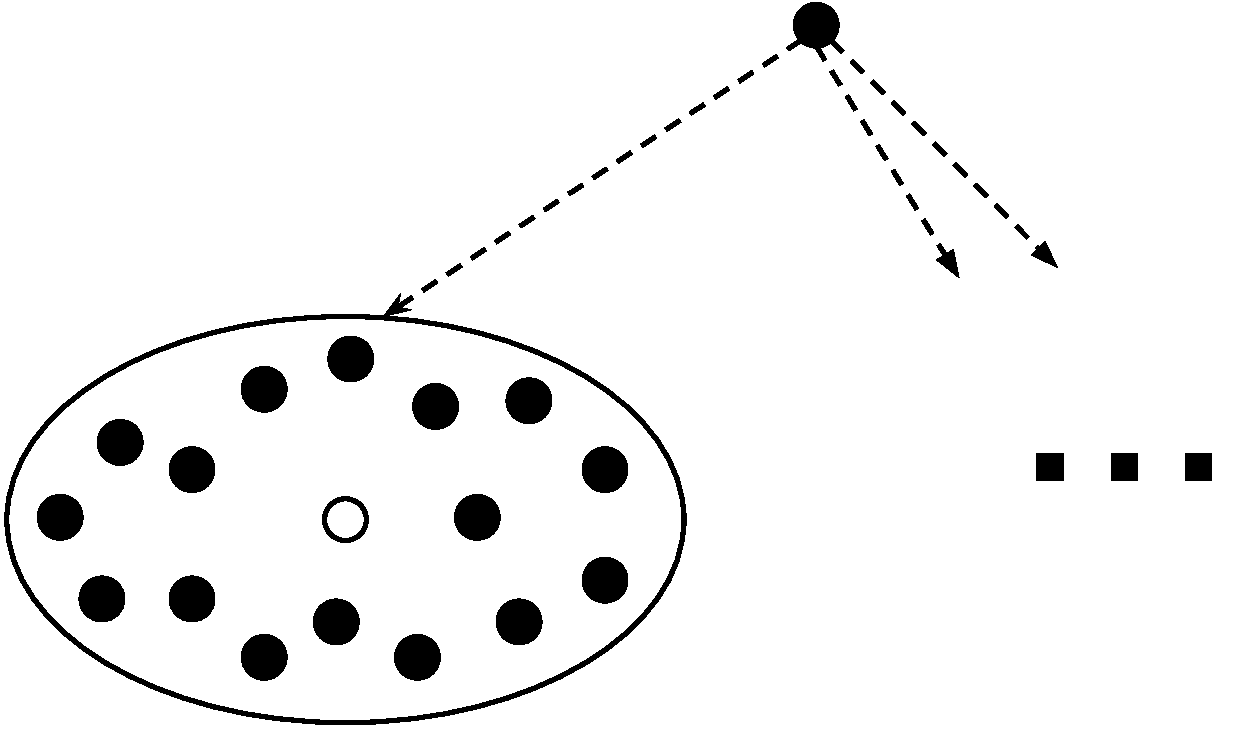
\includegraphics[scale=0.35]{PTree.pdf}
\caption{Graphical representation of $PTree$, $N$ Parallel work groups.}
\label{fig:PTree}
\end{figure}

\begin{figure}
\centering
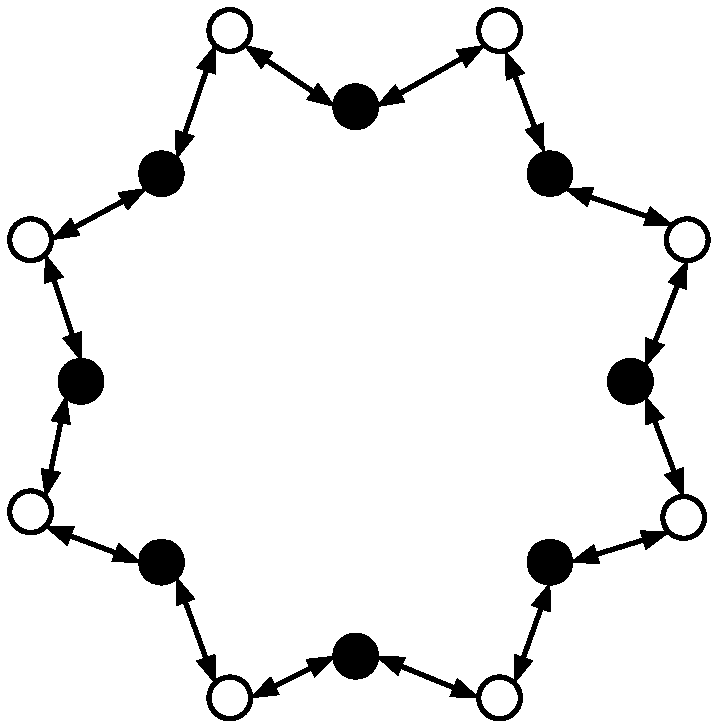
\includegraphics[scale=0.35]{PRing.pdf}
\caption{Graphical representation of $PRing$, full system predictable 
cooperation.}
\label{fig:PRing}
\end{figure}

\begin{figure}
\centering
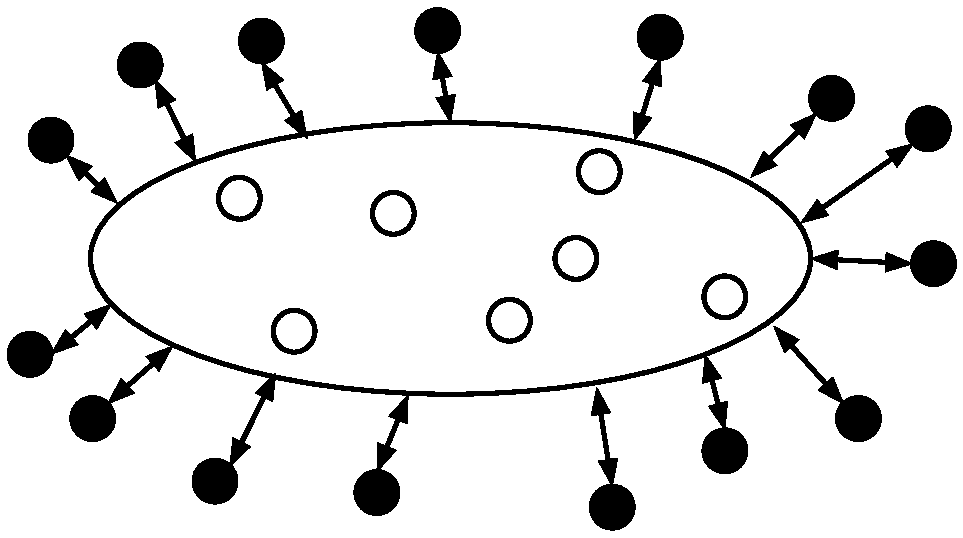
\includegraphics[scale=0.35]{ClusterComm.pdf}
\caption{Graphical representation of $ClusterComm$, $N$ processes to $M$ 
channels for unpredictable full system cooperation.}
\label{fig:ClusterComm}
\end{figure}

\begin{figure}
\centering
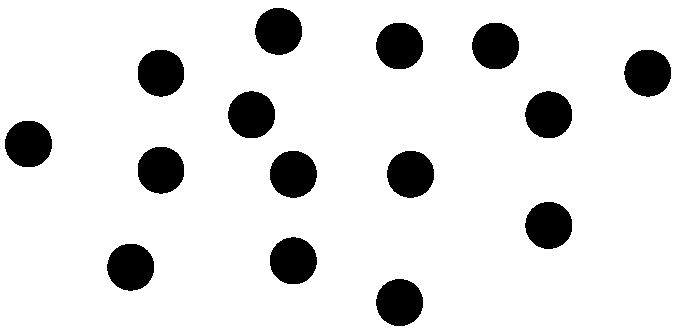
\includegraphics[scale=0.35]{ChugMachine.pdf}
\caption{Graphical representation of $ChugMachine$, $N$ worker processes 
without cooperation.}
\label{fig:}
\end{figure}

\begin{figure}
\centering
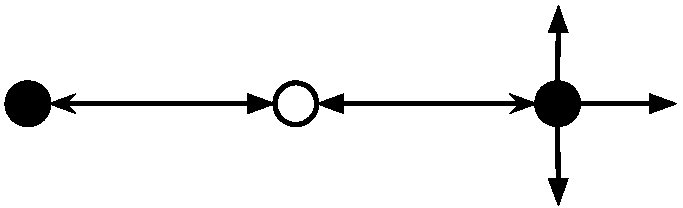
\includegraphics[scale=0.35]{UserInput.pdf}
\caption{Graphical representation of $UserInput$, single randomly hanging 
process.}
\label{fig:}
\end{figure}

\begin{figure}
\centering
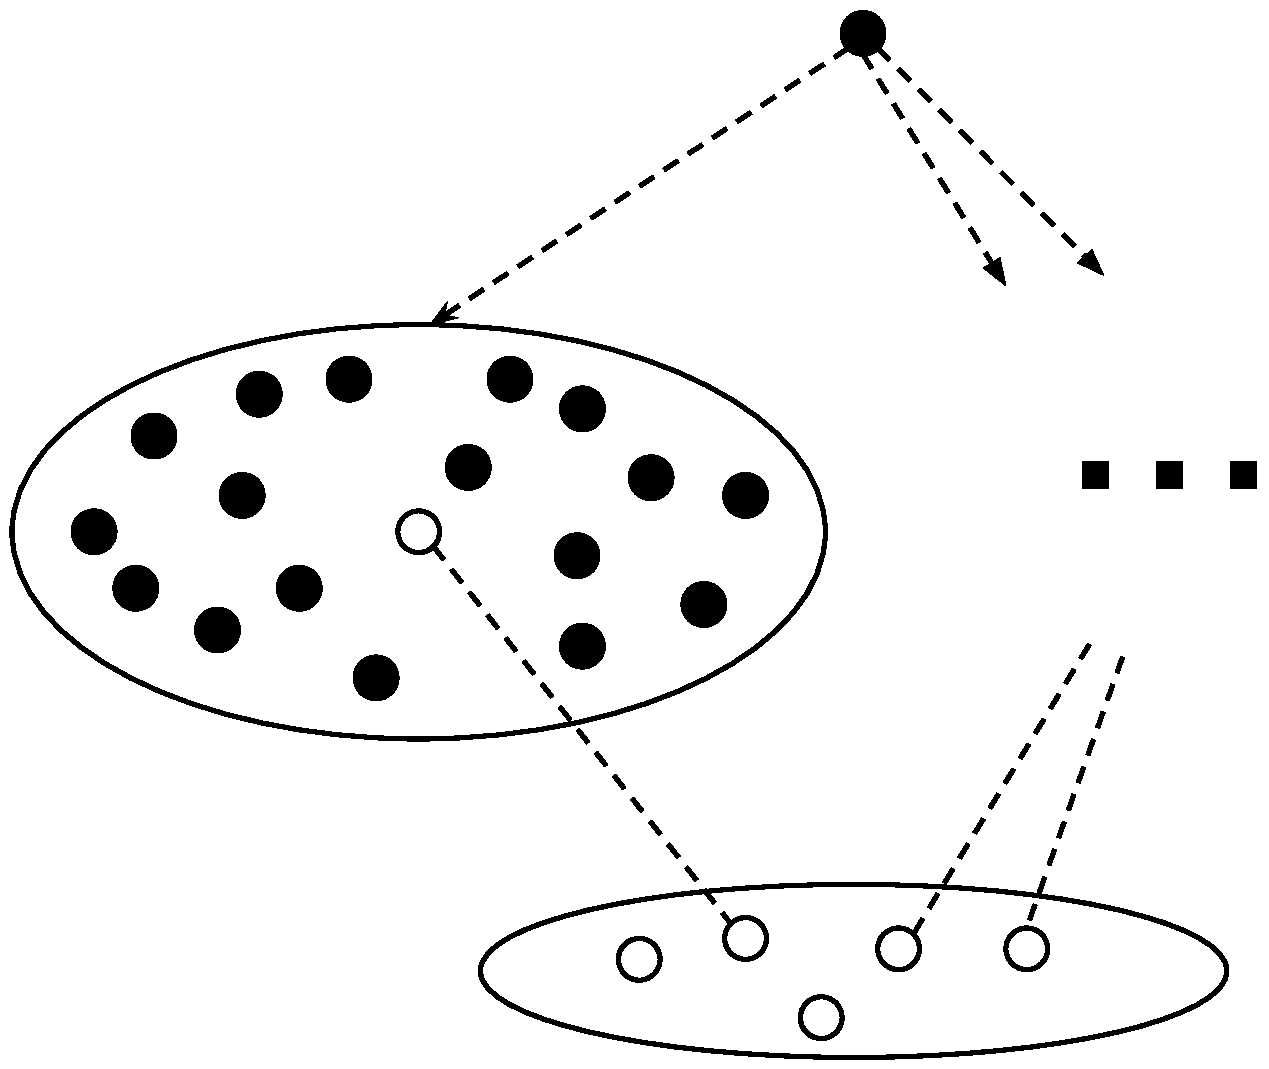
\includegraphics[scale=0.35]{JumpShip.pdf}
\caption{Graphical representation of $JumpShip$, $N$ Parallel phase shifting 
work groups.}
\label{fig:JumpShip}
\end{figure}





\section{Cooperativity Mechanics}\label{sec:cooperativity mechanics}

\subsection{Overview}\label{sec:cooperativity mechanics overview}
\subsection{Longevity-Based Batching}\label{sec:longevity based batching}
\subsection{Channel Pinning}\label{sec:channel pinning}
\subsection{Bipartite Graph Aided Shuffling}
    \label{sec:bipartite graph aided shuffling}


